\documentclass[10pt,a4paper]{article}
\usepackage[T1]{fontenc}
\usepackage[utf8]{inputenc}
\usepackage{graphicx}
\usepackage{tabularx}
\usepackage{helvet}
\usepackage{verbatim}
\usepackage{hyperref}
\usepackage[a4paper,margin=1in]{geometry}
\usepackage[polish]{babel}
\usepackage{float}

\renewcommand\familydefault{\sfdefault}

\begin{document}
\begin{titlepage}
	\centering
	{\Large Wydział Matematyki i Nauk Informacyjnych Politechniki Warszawskiej \par}
	\vspace{1cm}
	
\includegraphics[width=0.2\textwidth]{logo.png} \par
	\vspace{5cm}
	{\LARGE Chess3D -- wizualizacja gry w szachy \par}
	\vspace{0.5cm}
	{\Large Bartłomiej Dach \par}
	\vspace{1.5cm}
	{\Large Wersja 1.1 \par}
	\vspace{1.5cm}
	{\Large \today \par}
\end{titlepage}
Lista zmian w dokumencie:
\begin{table}[H]
\def\arraystretch{1.5}
\begin{tabularx}{\textwidth}{|l|l|X|l|}
	\hline
	\textbf{Data} & \textbf{Autor} & \textbf{Opis zmian} & \textbf{Wersja} \\
	\hline
	14.12.2016 & Bartłomiej Dach & Dodanie specyfikacji wymagań & 1.0 \\
	\hline
	15.12.2016 & Bartłomiej Dach & Rozszerzenie opisu biznesowego, dodanie szkicu architektury & 1.1 \\
	\hline
\end{tabularx}
\end{table}

\tableofcontents
\newpage

\section{Specyfikacja}

\subsection{Opis biznesowy}
Celem aplikacji \emph{Chess3D} jest wyświetlanie trójwymiarowej wizualizacji. Przedstawia ona scenę składającą się z szachownicy oraz pionków szachowych, oświetlanych światłem stożkowym.

Użytkownik aplikacji może zaznaczyć dowolny pionek na planszy, a następnie wskazywać pole, na który dany pionek powinien być przesunięty. Ruchy wykonane przez użytkownika nie muszą być prawidłowymi ruchami szachowymi, tj. ich poprawność pod tym kątem nie jest sprawdzana przez aplikację. Po wyspecyfikowaniu ruchu aplikacja w czasie rzeczywistym wyświetla animację przesunięcia pionka w nowe miejsce.

W zakresie projektu znajduje się również demonstracja kilku klasycznych metod symulacji światła dla obiektów trójwymiarowych, a mianowicie:
\begin{itemize}
	\item modele oświetlenia sceny:
	\begin{itemize}
		\item model Phonga \cite{phong75},
		\item model Blinna-Phonga \cite{blinn77},
	\end{itemize}
	\item tryby cieniowania trójkątów:
	\begin{itemize}
		\item cieniowanie płaskie,
		\item cieniowanie Gouraud \cite{gouraud71},
		\item cieniowanie Phonga \cite{phong75}.
	\end{itemize}
\end{itemize}
Użytkownik powinien mieć możliwość wyboru powyższych metod, skutkujący natychmiastową aktualizacją wyglądu sceny.

Dodatkowo, do wyboru przez użytkownika powinny być następujące trzy kamery, zmieniające perspektywę postrzegania sceny:
\begin{itemize}
	\item kamera nieruchoma, obejmująca całość szachownicy; usytuowanie tej kamery powinno umożliwiać łatwe wykonanie ruchu, czyli wybranie przez użytkownika pionka i pola,
	\item kamera nieruchoma, śledząca ruch ostatnio przesuniętego pionka,
	\item kamera ruchoma, związana z ostatnim poruszanym pionkiem na szachownicy.
\end{itemize}

Renderowanie sceny powinno odbywać się w trybie \emph{software}, tzn. obliczenia związane z wyświetlaniem obrazu mają używać procesora, zamiast jednostek \hyperref[abbr:gpu]{GPU}. Potok renderowania powinien być zaimplementowany od podstaw oraz wzorować się na istniejącym popularnym schemacie używanym w wielu bibliotekach graficznych 3D, takich, jak m.in. OpenGL, składającym się z następujących kroków:
\begin{itemize}
	\item transformacja współrzędnych (współrzędne świata, kamery),
	\item rzut na płaszczyznę,
	\item obcinanie wielokątów oraz eliminacja ścian tylnych,
	\item wypełnianie wielokątów zgodnie z przyjętym modelem oświetlenia.
\end{itemize}

\newpage

\subsection{Wymagania biznesowe}

\subsubsection*{Przypadki użycia}

Przypadki użycia aplikacji przedstawione są na poniższym diagramie UML.

\begin{figure}[H]
	\centering
	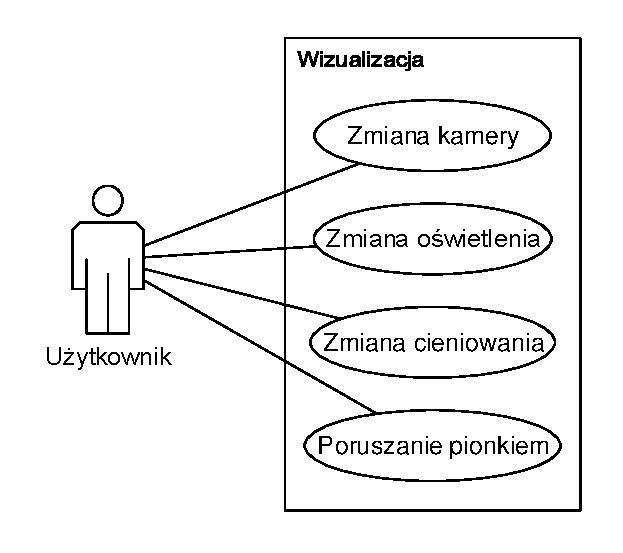
\includegraphics[width=7cm]{use-case.pdf}
	\caption{Diagram przypadków użycia}
\end{figure}

\begin{table}[H]
	\begin{tabularx}{\textwidth}{|l|X|X|}
		\hline
		\textbf{Nazwa} & \textbf{Opis} & \textbf{Odpowiedź systemu} \\
		\hline
		Zmiana kamery &
		Zmiana kamery w wizualizacji na jedną z trzech poniższych opcji:
		& Aktualizacja wizualizacji uwzględniająca wybór kamery.
		\\
		& $\bullet$ kamera nieruchoma, z widokiem na całą scenę, & \\
		& $\bullet$ kamera nieruchoma, śledząca ostatnio poruszony pionek, & \\
		& $\bullet$ kamera ruchoma, związana z ostatnio poruszonym pionkiem. & \\
		\hline
		Zmiana oświetlenia &
		Zmiana modelu oświetlenia sceny na model Phonga lub model Blinna. &
		Aktualizacja wizualizacji uwzględniająca wybrany model oświetlenia. \\
		\hline
		Zmiana cieniowania &
		Zmiana trybu cieniowania sceny na jeden z poniższych: &
		Aktualizacja wizualizacji uwzględniająca wybrany tryb cieniowania. \\
		& $\bullet$ cieniowanie stałe, & \\
		& $\bullet$ cieniowanie Gouraud, & \\
		& $\bullet$ cieniowanie Phonga. & \\
		\hline
		Poruszanie pionkiem &
		Przesunięcie pionka na nowe pole po wybraniu pionka i pola. &
		Animacja poruszania się pionka, wyświetlana w czasie rzeczywistym. \\
		\hline
	\end{tabularx}
	\caption{Opisy przypadków użycia}
\end{table}

\newpage

\subsection{Wymagania niefunkcjonalne}

W trakcie analizy rozpoznane zostały następujące wymagania niefunkcjonalne:

\begin{table}[H]
	\begin{tabularx}{\textwidth}{|l|X|}
		\hline
		\textbf{Obszar wymagań} & \textbf{Opis} \\
		\hline
		Użyteczność & Aplikacja powinna posiadać dwa tryby działania: okienkowy oraz pełnego ekranu. \\
		\hline
		Niezawodność & Na obrazie generowanym przez aplikację nie powinny być widoczne żadne artefakty lub zniekształcenia spowodowane błędami renderingu. \\
		\hline
		Wydajność & Aplikacja powinna być w stanie generować kolejne klatki obrazu w czasie krótszym niż 1 sekunda (płynność większa niż 1 klatka na sekundę). \\
		\cline{2-2}
		& Aplikacja powinna zajmować mniej niż 500 MB pamięci RAM systemu. \\
		\hline
		Utrzymanie & Wraz z aplikacją zostanie dołączona instrukcja obsługi. \\
		\cline{2-2}
		& Aplikacja będzie wspierała wczytywanie modeli pionków szachowych z plików \texttt{.obj} lub innych wspieranych przez narzędzia do modelowania 3D. \\
		\hline
	\end{tabularx}
	\caption{Lista wymagań niefunkcjonalnych dla aplikacji}
\end{table}

\subsection{Harmonogram projektu}

Harmonogram zadań przedstawiony jest na poniższym diagramie Gantta:

\begin{figure}[H]
	\centering
	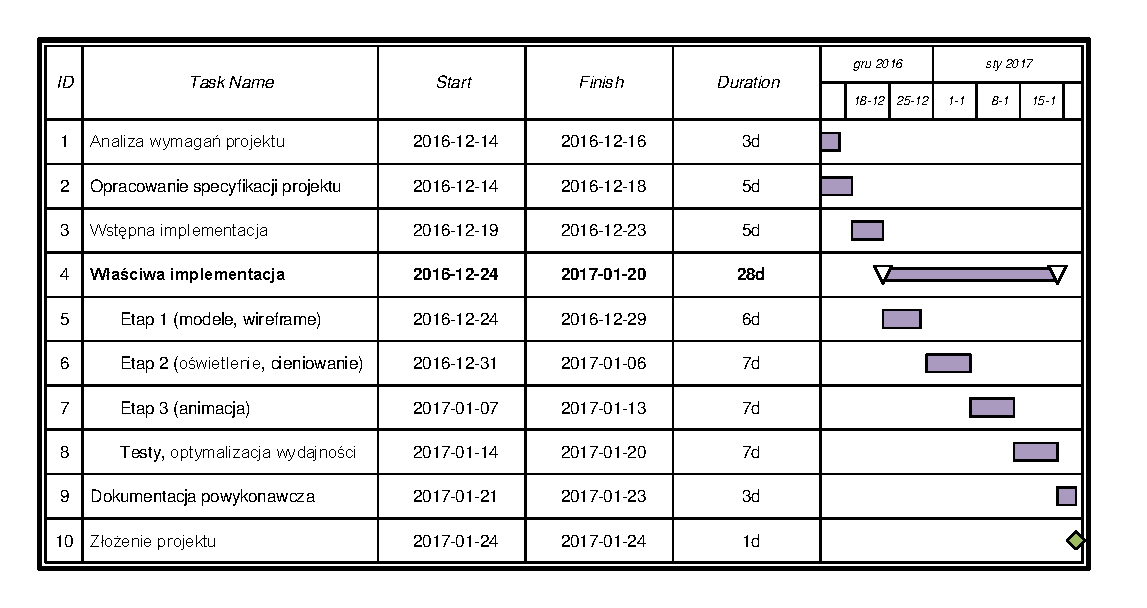
\includegraphics[width=14cm]{gantt-chart.pdf}
	\caption{Diagram Gantta przedstawiający planowany harmonogram prac}
\end{figure}
Poniżej przedstawione zostały kamienie milowe wchodzące w skład realizacji projektu.
\begin{enumerate}
	\item 16 grudnia 2016 -- zakończenie analizy wymagań projektu,
	\item 18 grudnia 2016 -- uzgodnienie specyfikacji projektu,
	\item 23 grudnia 2016 -- zakończenie wstępnej implementacji,
	\item 20 stycznia 2017 -- zakończenie właściwej implementacji,
	\item 23 stycznia 2017 -- zakończenie prac nad dokumentacją powykonawczą,
	\item 24 stycznia 2017 -- złożenie projektu wraz z pełną dokumentacją.
\end{enumerate}

\newpage

\subsection{Architektura rozwiązania}

Ze względu na spełniane funkcjonalności aplikacja została podzielona na komponenty w sposób zaprezentowany na poniższym diagramie:

\begin{figure}[H]
	\centering
	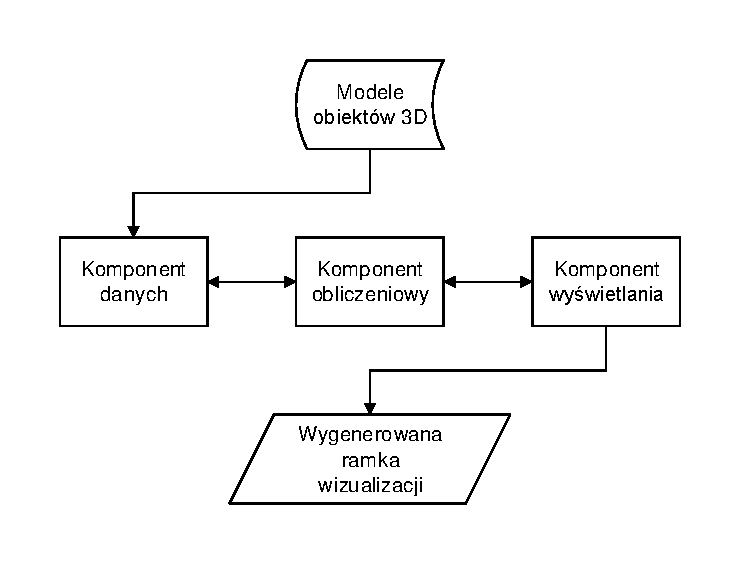
\includegraphics[width=10cm]{component-chart.pdf}
	\caption{Diagram komponentów aplikacji}
\end{figure}

\paragraph{Komponent danych}
Odpowiada za wczytanie z dysku danych związanych ze sceną, takich, jak: dane modeli wykorzystanych w scenie, położenie i parametry oświetlenia obiektów. Zawiera on również klasy reprezentujące te obiekty, których używa komponent obliczeniowy. Proces wczytywania modeli będzie wspomagany przez bibliotekę \emph{Assimp} \cite{assimp}.

\paragraph{Komponent obliczeniowy}
Jego rolą jest przetworzenie wczytanych z plików wejściowych danych i dokonanie właściwych obliczeń związanych z wizualizacją, tj. zmianę układów współrzędnych, rzutu na płaszczyznę oraz symulację oświetlenia. Do wykonywania obliczeń wykorzystana zostanie biblioteka \emph{Generic Graphics Toolkit} \cite{ggt}.

\paragraph{Komponent wyświetlania}
Wykorzystuje obliczenia wykonane przez powyższy komponent do właściwego tworzenia obrazu dwuwymiarowego i wyświetla go na ekranie. Ponadto obsługuje polecenia użytkownika, wydawane za pośrednictwem interfejsu graficznego, i przekazuje informacje o nich do pozostałych komponentów. W tym komponencie wykorzystane będą funkcjonalności biblioteki \emph{Simple DirectMedia Layer 2.0} \cite{sdl}.

W celu uzyskania jak największej wydajności, aplikacja tworzona będzie w języku C++.

\newpage

\begin{comment}
\section{Dokumentacja końcowa (powykonawcza)}

\subsection{Wymagania systemowe}
% Punkt obowiązkowy.
%
% Rozdział powinien zawierać wymagania systemowe, wymagane oprogramowanie zewnętrzne
% (RDBMS, etc.)

\subsection{Biblioteki wraz z określeniem licencji}
% Punkt obowiązkowy.
%
% Rozdział powinien zawierać listę użytych bibliotek i komponentów firm trzecich wraz z ich licencjami.

\subsection{Instrukcja instalacji}
% Punkt obowiązkowy.
%
% Niniejszy rozdział powinien kompletną instrukcję instalacji systemu/aplikacji umożliwiająca osobie
% oceniającej implementację danego rozwiązania. Uwaga: instrukcja powinna być dostoswana do
% instalacji na czystym systemie operacyjnym.

\subsection{Instrukcja uruchomienia}
% Punkt obowiązkowy.
% 
% Niniejszy rozdział powinien zawierać kompletną instrukcję uruchomienia systemu/aplikacji
% umożliwiającą osobie oceniającej weryfikację poprawności działania systemu.

\subsection{Instrukcja użycia}
% Punkt obowiązkowy.
%
% Niniejszy rozdział powinien zawierać kompletną instrukcję użycia (manual) systemu/aplikacji
% umożliwiająca osobie oceniającej weryfikację poprawności działania systemu.

\subsection{Instrukcja utrzymania}
% Punkt obowiązkowy.
%
% Niniejszy rozdział powinien zawierać kompletną instrukcję utrzymania systemu obejmującą procedury
% włączenia, wyłączenia systemu oraz procedury backup/restore.

\subsection{Raport odstępstw od specyfikacji wymagań}
% Punkt obowiązkowy.

\subsection{Dokumentacja usług Web Services}
% Punkt obowiązkowy
%
% Niniejszy rozdział powinien w przypadku, gdy system udostępnia publiczne usługi web services
% powinien zawierać dokumentację usług zamieszczone w formie opisowej lub np. wg specyfikacji
% swagger.

\section{Dokumentacja końcowa (powykonawcza) -- punkty wymagane przez prowadzącego zajęcia}

\subsection{Pseudokod}

\subsection{Diagramy sekwencji}
% Punkt obowiązkowy
%
% W przypadku projektów półsemestralnych lub dłuższych: w przypadku, gdy system składa się z
% komponentów rozproszonych należy dołączyć diagram(y) sekwencji. Rozdział zawierać powinien
% zawierać diagramy sekwencji opisujące komunikację pomiędzy systemami lub komponentami
% systemu. Należy w nim uwzględnić wszystkie przepływy komunikatów pomiędzy komponentami
% systemu lub systemami.

\subsection{Model danych}
% W przypadku projektów półsemestralnych lub dłuższych, gdy system składuje dane, należy opisać
% model danych. Model danych powinien być wyrażony przez diagram entity relationship w przypadku
% relacyjnej bazy danych. Zalecane jest wówczas opisanie znaczenia poszczególnych relacji, jak
% również czytelne oznaczenie rodzaju relacji (np. jeden do wielu) oraz kluczy głównych i kluczy obcych.
% W przypadku wykorzystania platform nierelacyjnych np. platform NoSQL lub składowania danych w
% plikach Apache Hadoop należy przedstawić opis konwencji zapisu danych. Jest to szczególnie istotne,
% gdy model danych jest prowadzony w trybie tzw. schema-on-read tzn. nie jest egzekwowany przez
% platformę składowania danych, a zależy wyłącznie od konwencji stosowanej przez aplikację np.
% konwencji nazewnictwa kolumn, treści wpisów w formacie JSON lub formatu sekwencji plików
% tworzonych w systemie plików HDFS.

\subsection{Scenariusz testów akceptacyjnych}
% W przypadku projektów półsemestralnych np. realizowanych w ramach projektu zespołowego.
% Rozdział powinien zawierać scenariusze testów akceptacyjnych nawiązujących do wymagań
% funkcjonalnych i niefunkcjonalnych systemu.

\subsection{Raport z przeprowadzonych testów}
% W przypadku projektów półsemestralnych np. realizowanych w ramach projektu zespołowego.
% Rozdział powinien zawierać scenariusze testów akceptacyjnych nawiązujących do wymagań
% funkcjonalnych i niefunkcjonalnych systemu i wyniki ich przeprowadzenia.
\end{comment}

\section{Lista użytych skrótów}

\label{abbr:gpu}
\paragraph{GPU} Graphics Processing Unit

\renewcommand*{\refname}{\vspace*{-2em}}
\section{Bibliografia}
\begin{thebibliography}{99}

\bibitem{assimp}
	Assimp -- Open Asset Import Library,
	\url{http://www.assimp.org/}

\bibitem{blinn77}
	James F. Blinn,
	\emph{Models of Light Reflection for Computer Synthesized Pictures},
	Proceedings of the 4th Annual Conference on Computer Graphics and Interactive Techniques,
	pp. 192-198.

\bibitem{ggt}
	Generic Graphics Toolkit,
	\url{http://ggt.sourceforge.net/}
	
\bibitem{gouraud71}
	Henri Gouraud,
	\emph{Continuous Shading of Curved Surfaces},
	IEEE Transactions on Computers,
	June 1971, Volume C-20, Number 6,
	pp. 87-93.

\bibitem{phong75}
	Bui Tuong Phong,
	\emph{Illumination for Computer Generated Pictures},
	Communications of the ACM,
	June 1975, Volume 18, Number 6,
	pp. 311-317.

\bibitem{sdl}
	Simple DirectMedia Layer,
	\url{https://www.libsdl.org/}
\end{thebibliography}
\end{document}